\documentclass[11pt,a4paper]{ctexart}

% =====================================================
% Standard Preamble & ipara Package
% =====================================================
\usepackage[teacher]{../../ipara}
\usepackage{mathtools}
\usetikzlibrary{calc,arrows.meta,positioning}

\definecolor{rulecolor}{RGB}{90,105,125}
\definecolor{teachblue}{RGB}{32,91,161}
\definecolor{softblue}{RGB}{239,246,253}
\definecolor{softgray}{RGB}{247,248,250}
\definecolor{softorange}{RGB}{255,247,235}

\columnratio{0.5}

\setlength{\parindent}{0pt}
\setlength{\parskip}{0.35em}
\setlist[itemize]{leftmargin=2em,itemsep=0.1em,topsep=0.2em}
\setlist[enumerate]{leftmargin=2em,itemsep=0.1em,topsep=0.2em}

\providecommand{\teachbox}[1]{
  \begin{tcolorbox}[enhanced,breakable,colback=softblue,colframe=teachblue,
    boxrule=0.7pt,arc=1.2mm,left=1.4mm,right=1.4mm,top=1.2mm,bottom=1.2mm,
    title={#1},fonttitle=\bfseries]
  \end{tcolorbox}
}
\providecommand{\teachblock}[2]{%
  \begin{tcolorbox}[enhanced,breakable,colback=white,colframe=rulecolor,
    boxrule=0.55pt,arc=1mm,left=1.4mm,right=1.4mm,top=1.1mm,bottom=1.1mm,
    title={#1},fonttitle=\bfseries]
  #2
  \end{tcolorbox}
}
\providecommand{\teachquestionheader}[1]{%
  \vspace{0.4em}
  \begin{tcolorbox}[colback=softgray,colframe=rulecolor,boxrule=0.6pt,arc=0.8mm,
    left=1.2mm,right=1.2mm,top=0.8mm,bottom=0.8mm]
    \bfseries #1
  \end{tcolorbox}
}
\providecommand{\mcoptions}[4]{%
  \begin{tabularx}{\linewidth}{@{}X X@{}}
  A. #1 & B. #2 \\
  C. #3 & D. #4
  \end{tabularx}
}
\providecommand{\mcfigurequestion}[3]{%
  \begin{minipage}[t]{0.67\textwidth}
    #1\par\vspace{0.4em}#2
  \end{minipage}\hfill
  \begin{minipage}[t]{0.29\textwidth}
    \centering #3
  \end{minipage}
}
\providecommand{\answerblank}[1][3.5cm]{%
  \begin{tcolorbox}[colback=white,colframe=rulecolor!65,boxrule=0.45pt,arc=0.8mm,
    title={作答区},fonttitle=\bfseries]
    \vspace{#1}
  \end{tcolorbox}
}

% Parallel-projection basis used by the major 3D figures.
% Every large-example diagram below is generated from genuine 3D coordinates.
\tikzset{spatial/.style={
  x={(0.95cm,-0.10cm)},
  y={(0.48cm,0.34cm)},
  z={(0cm,0.88cm)},
  >=Stealth,line join=round,line cap=round
}}

% =====================================================
% Header / footer
% =====================================================
\pagestyle{fancy}
\fancyhf{}
\lhead{\small 公共专题教案：第一讲·线面平行垂直与书写规范}
\rhead{\small 教师版}
\cfoot{\small 第 \thepage\ 页\quad 共 \pageref{LastPage} 页}
\renewcommand{\headrulewidth}{0.4pt}
\renewcommand{\footrulewidth}{0pt}
\begin{document}

\begin{center}
  {\Large\bfseries 第一讲：立体几何——线面平行垂直与书写规范}\par
  \vspace{0.3em}
  {\large 公共专题课：把空间关系翻译成无扣分的完整证明链}\par
  \vspace{0.3em}
  {\small 课时：120 分钟\quad （附录 A：建系与空间向量通用体系·课后进阶）}
\end{center}

% =====================================================
% 课程定位
% =====================================================
\section{课程定位与 120 分钟流程}

\begin{teachbox}{本节课的定位}
立体几何第一问的核心不是"看出答案"，而是"把看出来的关系写成无扣分的证明链"。

很多学生不是不会做，而是：
\begin{itemize}[leftmargin=2em, itemsep=0.1em]
  \item 证明线面垂直时，漏写"两条直线在目标平面内且相交"；
  \item 证明线面平行时，漏写"直线不在平面内"；
  \item 证明面面垂直性质时，漏写"交线"；
  \item 习惯机械套公式，无法把图上的几何特征（如中点、平行四边形、等腰三角形中线）准确翻译成定理前提。
\end{itemize}

本节课的目标：\textbf{用 120 分钟，把学生从“凭感觉画辅助线”训练成“按得分句写证明”。}
\end{teachbox}

\vspace{0.4em}
\begin{tabularx}{\textwidth}{p{3.2cm}p{4.5cm}X}
\toprule
时间 & 教学环节 & 核心动作 / 检查点 \\
\midrule
0--10 分钟 & 核心观念与定理激活 & 快速复习 8 大基本定理，强调每一个定理“最容易漏掉的条件”。 \\ \hline
10--25 分钟 & 应试书写规范（得分句） & 明确 5 个标准得分句模板，强调“归属、相交、排除、定理链”四步自查。 \\ \hline
25--45 分钟 & 选择题易错判断（6 题） & 课堂精讲 6 道判断题，重点纠正“只差一个词就错”的逻辑漏洞。 \\ \hline
45--65 分钟 & 例 1：直接线面平行 & 训练基本中位线直接平移行，明确部分几何度量条件为第二问建系备用。 \\ \hline
65--85 分钟 & 例 2：辅助面面平行法 & 训练“一条线不好找，就补中点构造平行平面”的升阶技巧。 \\ \hline
85--100 分钟 & 例 3：纯几何线面垂直 & 训练“等腰三角形中线 + 面面垂直性质 + 平行四边形中点”链条。 \\ \hline
100--112 分钟 & 例 4：数量关系反推垂直 & 训练“体积反推线段长 $\to$ 等腰直角三角形 $\to$ 综合垂直证明”。 \\ \hline
112--120 分钟 & 总结与收束 & 四句总结 + 得分句默写 + 课后复练安排。 \\
\bottomrule
\end{tabularx}
\vspace{0.4em}
\textbf{注}：立体几何第二问向量计算及通用建系技巧收录于《附录 A：建系与空间直角坐标系（向量法通用体系）》，作为课后进阶与第二讲备课资料。

% =====================================================
% 第一板块：核心观念与定理
% =====================================================
\section{核心观念与基本定理}

\teachblock{核心观念：立体几何不是"看图"，而是"翻译"}{
立体几何证明本质上是把图形关系写成数学条件链：
\[
  l\subset\alpha,\quad l\parallel m,\quad l\perp\alpha,\quad \alpha\cap\beta=m
\]
\textbf{看出来不等于证明出来。}证明题中必须把定理的前提条件写完整。

课堂上可以追问："你说这两条线垂直，那它们分别在哪个平面内？交于哪个点？"如果答不出来，就说明“看出来了但翻译不出来”。
}

\subsection{平行关系定理}

\teachblock{定理 1：线面平行判定}{
\begin{minipage}[c]{0.66\textwidth}
  若 $m\subset\alpha$，$l\parallel m$，且 $l\not\subset\alpha$，则 $l\parallel\alpha$。
  
  \textbf{最容易漏掉的}：$l\not\subset\alpha$。若 $l\subset\alpha$，则不能写 $l\parallel\alpha$。
\end{minipage}%
\hfill
\begin{minipage}[c]{0.32\textwidth}
  \centering
  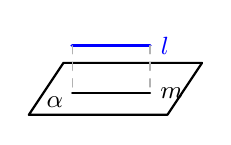
\begin{tikzpicture}[scale=0.55, >=stealth, line join=round, line cap=round]
    \draw[thick] (0,0) -- (3.2,0) -- (4.0,1.2) -- (0.8,1.2) -- cycle;
    \node at (0.6, 0.3) {\small $\alpha$};
    \draw[thick] (1.0, 0.5) -- (2.8, 0.5) node[right]{\small $m$};
    \draw[very thick, blue] (1.0, 1.6) -- (2.8, 1.6) node[right]{\small $l$};
    \draw[dashed, gray!60] (1.0, 1.6) -- (1.0, 0.5);
    \draw[dashed, gray!60] (2.8, 1.6) -- (2.8, 0.5);
  \end{tikzpicture}
\end{minipage}
}

\teachblock{定理 2：线面平行性质}{
\begin{minipage}[c]{0.66\textwidth}
  若 $l\parallel\alpha$，$l\subset\beta$，$\alpha\cap\beta=m$，则 $l\parallel m$。
  
  \textbf{关键是找交线}：过该直线的平面与已知平面的交线，必与该直线平行。
\end{minipage}%
\hfill
\begin{minipage}[c]{0.32\textwidth}
  \centering
  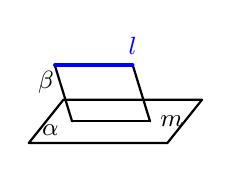
\begin{tikzpicture}[scale=0.55, >=stealth, line join=round, line cap=round]
    \draw[thick] (0,0) -- (3.2,0) -- (4.0,1.0) -- (0.8,1.0) -- cycle;
    \node at (0.5, 0.3) {\small $\alpha$};
    \draw[thick] (1.0, 0.5) -- (2.8, 0.5) node[right]{\small $m$};
    \draw[thick] (1.0, 0.5) -- (0.6, 1.8) -- (2.4, 1.8) -- (2.8, 0.5);
    \node at (0.4, 1.4) {\small $\beta$};
    \draw[very thick, blue] (0.6, 1.8) -- (2.4, 1.8) node[above]{\small $l$};
  \end{tikzpicture}
\end{minipage}
}

\teachblock{定理 3：面面平行判定}{
\begin{minipage}[c]{0.66\textwidth}
  若 $a\subset\beta$，$b\subset\beta$，$a\cap b=O$，且 $a\parallel\alpha$，$b\parallel\alpha$，则 $\beta\parallel\alpha$。

  \textbf{常用推论}：若 $a,b\subset\beta$ 相交，$a',b'\subset\alpha$ 相交，且 $a\parallel a'$、$b\parallel b'$，则 $\beta\parallel\alpha$。

  \textbf{必须注意}：核心条件是同一平面内的\textbf{两条相交直线}，不能只凭“两条线都平行于同一平面”下结论。
\end{minipage}%
\hfill
\begin{minipage}[c]{0.32\textwidth}
  \centering
  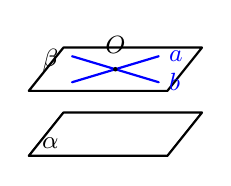
\begin{tikzpicture}[scale=0.55, >=stealth, line join=round, line cap=round]
    \draw[thick] (0,0) -- (3.2,0) -- (4.0,1.0) -- (0.8,1.0) -- cycle;
    \node at (0.5, 0.3) {\small $\alpha$};
    \draw[thick] (0,1.5) -- (3.2,1.5) -- (4.0,2.5) -- (0.8,2.5) -- cycle;
    \node at (0.5, 2.2) {\small $\beta$};
    \draw[thick, blue] (1.0, 1.7) -- (3.0, 2.3) node[right]{\small $a$};
    \draw[thick, blue] (1.0, 2.3) -- (3.0, 1.7) node[right]{\small $b$};
    \fill (2.0, 2.0) circle (1.5pt) node[above=2pt] {\small $O$};
  \end{tikzpicture}
\end{minipage}
}

\teachblock{定理 4：面面平行性质}{
\begin{minipage}[c]{0.66\textwidth}
  若 $\alpha\parallel\beta$，$l\subset\alpha$，则 $l\parallel\beta$。
  
  若 $\alpha\parallel\beta$，$l\perp\alpha$，则 $l\perp\beta$。
\end{minipage}%
\hfill
\begin{minipage}[c]{0.32\textwidth}
  \centering
  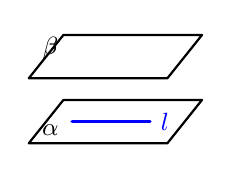
\begin{tikzpicture}[scale=0.55, >=stealth, line join=round, line cap=round]
    \draw[thick] (0,0) -- (3.2,0) -- (4.0,1.0) -- (0.8,1.0) -- cycle;
    \node at (0.5, 0.3) {\small $\alpha$};
    \draw[thick] (0,1.5) -- (3.2,1.5) -- (4.0,2.5) -- (0.8,2.5) -- cycle;
    \node at (0.5, 2.2) {\small $\beta$};
    \draw[very thick, blue] (1.0, 0.5) -- (2.8, 0.5) node[right]{\small $l$};
  \end{tikzpicture}
\end{minipage}
}

\subsection{垂直关系定理}

\teachblock{定理 5：线面垂直判定}{
\begin{minipage}[c]{0.66\textwidth}
  若 $a\subset\alpha$，$b\subset\alpha$，$a\cap b=O$，且 $l\perp a$，$l\perp b$，则 $l\perp\alpha$。
  
  \textbf{必须强调"在目标平面内且相交"}。若 $a\parallel b$，即使 $l$ 同时垂直于 $a,b$，也不能推出 $l\perp\alpha$。
\end{minipage}%
\hfill
\begin{minipage}[c]{0.32\textwidth}
  \centering
  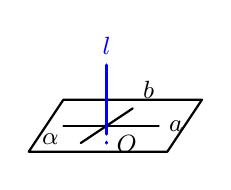
\begin{tikzpicture}[scale=0.55, >=stealth, line join=round, line cap=round]
    \draw[thick] (0,0) -- (3.2,0) -- (4.0,1.2) -- (0.8,1.2) -- cycle;
    \node at (0.5, 0.3) {\small $\alpha$};
    \draw[thick] (0.8, 0.6) -- (3.0, 0.6) node[right]{\small $a$};
    \draw[thick] (1.2, 0.2) -- (2.4, 1.0) node[above right]{\small $b$};
    \fill (1.8, 0.6) circle (1.5pt) node[below right] {\small $O$};
    \draw[very thick, blue] (1.8, 0.6) -- (1.8, 2.0) node[above]{\small $l$};
    \draw[dashed, very thick, blue] (1.8, 0.6) -- (1.8, 0.2);
  \end{tikzpicture}
\end{minipage}
}

\teachblock{定理 6：线面垂直性质}{
\begin{minipage}[c]{0.66\textwidth}
  若 $l\perp\alpha$，$a\subset\alpha$，则 $l\perp a$。
  
  \textbf{证明线线垂直的常用路线}：先证明某条线垂直于一个平面，再推出它垂直于该平面内的任意直线。
\end{minipage}%
\hfill
\begin{minipage}[c]{0.32\textwidth}
  \centering
  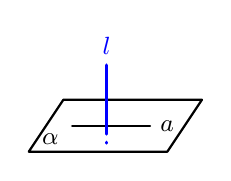
\begin{tikzpicture}[scale=0.55, >=stealth, line join=round, line cap=round]
    \draw[thick] (0,0) -- (3.2,0) -- (4.0,1.2) -- (0.8,1.2) -- cycle;
    \node at (0.5, 0.3) {\small $\alpha$};
    \draw[thick] (1.0, 0.6) -- (2.8, 0.6) node[right]{\small $a$};
    \draw[very thick, blue] (1.8, 0.6) -- (1.8, 2.0) node[above]{\small $l$};
    \draw[dashed, very thick, blue] (1.8, 0.6) -- (1.8, 0.2);
  \end{tikzpicture}
\end{minipage}
}

\teachblock{定理 7：面面垂直判定}{
\begin{minipage}[c]{0.66\textwidth}
  若 $l\subset\beta$，$l\perp\alpha$，则 $\beta\perp\alpha$。
  
  \textbf{常用思路}：在其中一个平面内找到一条直线，使它垂直于另一个平面。
\end{minipage}%
\hfill
\begin{minipage}[c]{0.32\textwidth}
  \centering
  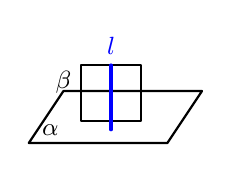
\begin{tikzpicture}[scale=0.55, >=stealth, line join=round, line cap=round]
    \draw[thick] (0,0) -- (3.2,0) -- (4.0,1.2) -- (0.8,1.2) -- cycle;
    \node at (0.5, 0.3) {\small $\alpha$};
    \draw[thick] (1.2, 0.5) -- (1.2, 1.8) -- (2.6, 1.8) -- (2.6, 0.5) -- cycle;
    \node at (0.8, 1.4) {\small $\beta$};
    \draw[very thick, blue] (1.9, 0.5) -- (1.9, 1.8) node[above]{\small $l$};
    \draw[dashed, very thick, blue] (1.9, 0.5) -- (1.9, 0.2);
  \end{tikzpicture}
\end{minipage}
}

\teachblock{定理 8：面面垂直性质}{
\begin{minipage}[c]{0.66\textwidth}
  若 $\alpha\perp\beta$，$\alpha\cap\beta=m$，且 $l\subset\alpha$，$l\perp m$，则 $l\perp\beta$。
\end{minipage}%
\hfill
\begin{minipage}[c]{0.32\textwidth}
  \centering
  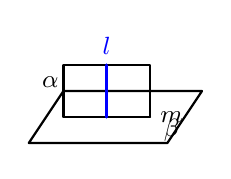
\begin{tikzpicture}[scale=0.55, >=stealth, line join=round, line cap=round]
    \draw[thick] (0,0) -- (3.2,0) -- (4.0,1.2) -- (0.8,1.2) -- cycle;
    \node at (3.3, 0.3) {\small $\beta$};
    \draw[thick] (0.8, 0.6) -- (2.8, 0.6) node[right]{\small $m$};
    \draw[thick] (0.8, 0.6) -- (0.8, 1.8) -- (2.8, 1.8) -- (2.8, 0.6) -- cycle;
    \node at (0.5, 1.4) {\small $\alpha$};
    \draw[very thick, blue] (1.8, 0.6) -- (1.8, 1.8) node[above]{\small $l$};
  \end{tikzpicture}
\end{minipage}
}

\teachblock{二级结论：两个垂直平面的交线}{
\begin{minipage}[c]{0.66\textwidth}
  若两个相交平面都垂直于同一个平面，则它们的交线垂直于这个平面。
  \[
    \alpha\perp\gamma,\quad \beta\perp\gamma,\quad \alpha\cap\beta=l
    \Rightarrow l\perp\gamma.
  \]
  \textbf{图形检查}：两个竖直平面在底面 $\gamma$ 上的交线方向必须不同；若画成同一方向，就会把两个平面误画成同一个平面。
\end{minipage}%
\hfill
\begin{minipage}[c]{0.32\textwidth}
  \centering
  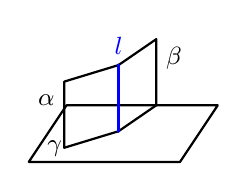
\begin{tikzpicture}[scale=0.60,>=Stealth,line join=round,line cap=round]
    \coordinate (O) at (1.9,0.65);
    \coordinate (U) at (0.75,0.30);
    \coordinate (V) at (2.70,1.20);
    \coordinate (Z) at (1.9,2.05);
    \draw[thick] (0,0)--(3.2,0)--(4.0,1.2)--(0.8,1.2)--cycle;
    \node at (0.55,0.28){\small $\gamma$};
    \draw[thick] (O)--(U);
    \draw[thick] (O)--(V);
    \draw[thick] (U)--($(U)+(0,1.4)$)--(Z)--(O);
    \draw[thick] (V)--($(V)+(0,1.4)$)--(Z)--(O);
    \node[left] at ($(U)+(0,1.0)$){\small $\alpha$};
    \node[right] at ($(V)+(0,1.0)$){\small $\beta$};
    \draw[very thick,blue] (O)--(Z) node[above]{\small $l$};
  \end{tikzpicture}
\end{minipage}
}

\teachblock{看到条件，立刻想到什么}{
\begin{itemize}
  \item 看到"证明线面平行"$\to$在目标平面内找一条与已知直线平行的直线。
  \item 看到"证明面面平行"$\to$在一个平面内找两条相交直线，分别平行于另一个平面。
  \item 看到"中点""三等分点"$\to$中位线、平行四边形、相似或向量比例。
  \item 看到"证明线线垂直"$\to$先证明其中一条线垂直于某个平面。
  \item 看到"证明面面垂直"$\to$在一个平面内找一条线垂直于另一个平面。
  \item 看到"两个平面垂直且给出交线"$\to$在一个平面内找垂直交线的直线，推出它垂直另一个平面。
\end{itemize}
}

% =====================================================
% 第二板块：应试书写规范（先定标准，再做题）
% =====================================================
\section{应试书写规范：先把“得分句”定下来}

\teachblock{为什么这一板块必须提前}{
本讲不是“会看图就行”，而是训练学生把空间关系写成阅卷可识别的完整逻辑链。后面的每一道选择题和证明题，都按下面的模板检查前提。
}

\begin{tabularx}{\textwidth}{p{3.2cm}X}
\toprule
目标 & 标准得分句 / 必查前提 \\
\midrule
线面平行 & $m\subset\alpha,\ l\parallel m,\ l\not\subset\alpha\Rightarrow l\parallel\alpha$。最容易漏：$l\not\subset\alpha$。 \\ \hline
线面垂直 & $a,b\subset\alpha,\ a\cap b=O,\ l\perp a,\ l\perp b\Rightarrow l\perp\alpha$。最容易漏：$a,b$ 在目标平面内且相交。 \\ \hline
面面平行 & 在同一平面内找两条相交直线，分别与另一平面平行；或分别平行于另一平面内两条相交直线。 \\ \hline
面面垂直 & 在其中一个平面内找到一条直线 $l$，证明 $l\perp$ 另一个平面。 \\ \hline
面面垂直性质 & 必须写出交线：$\alpha\perp\beta,\ \alpha\cap\beta=m,\ l\subset\alpha,\ l\perp m\Rightarrow l\perp\beta$。 \\
\bottomrule
\end{tabularx}

\begin{teachbox}{四步自查：每次写完证明后都扫一遍}
\begin{enumerate}[label=\arabic*.]
  \item \textbf{归属}：关键直线是否明确写了属于哪个平面？
  \item \textbf{相交}：线面垂直、面面平行中用到的两条直线是否明确相交？
  \item \textbf{排除}：证明线面平行时，是否排除了直线在平面内？
  \item \textbf{定理链}：每一个“所以”前面，是否已经凑齐对应定理的全部前提？
\end{enumerate}
\end{teachbox}

% =====================================================
% 第三板块：选择题易错判断（课堂精选 6 题）
% =====================================================
\section{选择题易错判断：6 道核心题}

\teachblock{板块目标}{
每道题都要求学生先说“使用了哪条定理”，再说“哪个前提缺失或哪个反例可以击破”。课堂不追求刷题数量，只训练定理前提检查。
}

% --- 选择 1 ---
\teachquestionheader{选择 1：面面垂直与线面垂直}
\mcfigurequestion{已知互相垂直的两个平面 $\alpha,\beta$ 交于直线 $l$，若直线 $m$ 满足 $m\perp\alpha$，则下列结论正确的是}{
  \mcoptions{$m\perp\beta$}{$m\perp l$}{$m\parallel\beta$}{$m\parallel l$}
}{
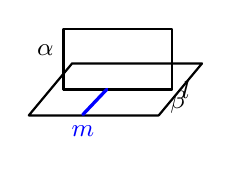
\begin{tikzpicture}[scale=0.55,>=Stealth,line join=round,line cap=round]
  \draw[thick] (0,0)--(3.0,0)--(4.0,1.2)--(1.0,1.2)--cycle;
  \node at (3.45,0.3){\small $\beta$};
  \draw[thick] (0.8,0.6)--(3.3,0.6)--(3.3,2.0)--(0.8,2.0)--cycle;
  \node[left] at (0.8,1.5){\small $\alpha$};
  \draw[thick] (0.8,0.6)--(3.3,0.6) node[right]{\small $l$};
  \coordinate(F) at (1.8,0.6);
  \draw[very thick,blue] (F)--(1.25,0.02) node[below]{\small $m$};
\end{tikzpicture}}

\begin{paracol}{2}
\teachblock{标准结论}{\textbf{答案 B}。$m\perp\alpha$ 说明 $m$ 垂直于 $\alpha$ 内任何直线。因为 $l\subset\alpha$，所以必然有 $m\perp l$。}
\switchcolumn
\teachblock{错项点拨}{A 项：$m$ 可能平行于 $\beta$；C 项：$m$ 也可能在 $\beta$ 内；D 项：$m\perp l$ 而非平行。}
\end{paracol}


% --- 选择 2 ---
\teachquestionheader{选择 2：基本命题真假判断}
\mcfigurequestion{设 $\alpha,\beta$ 是互不重合的平面，$l,m,n$ 是互不重合的直线，下列命题正确的是}{
\mcoptions
{若 $m,n\subset\alpha$，$l\perp m$，$l\perp n$，则 $l\perp\alpha$}
{若 $l\perp m$，$l\perp n$，则 $m\parallel n$}
{若 $l\parallel\alpha$，$m\parallel\beta$，$\alpha\perp\beta$，则 $l\perp m$}
{若 $l\perp\alpha$，$l\parallel\beta$，则 $\alpha\perp\beta$}
}{
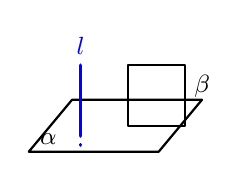
\begin{tikzpicture}[scale=0.55,>=Stealth,line join=round,line cap=round]
  \draw[thick] (0,0)--(3.0,0)--(4.0,1.2)--(1.0,1.2)--cycle;
  \node at (0.45,0.3){\small $\alpha$};
  \draw[thick] (2.3,0.6)--(2.3,2.0)--(3.6,2.0)--(3.6,0.6)--cycle;
  \node[right] at (3.6,1.5){\small $\beta$};
  \draw[very thick,blue] (1.2,0.55)--(1.2,2.0) node[above]{\small $l$};
  \draw[dashed,very thick,blue] (1.2,0.55)--(1.2,0.15);
\end{tikzpicture}}

\begin{paracol}{2}
\teachblock{标准结论}{\textbf{答案 D}。若 $l\perp\alpha$，$l\parallel\beta$，可在 $\beta$ 内取 $l'\parallel l$，得 $l'\perp\alpha$，而 $l'\subset\beta$，故由面面垂直判定可得 $\alpha\perp\beta$。}
\switchcolumn
\teachblock{错项点拨}{A 项缺少“$m,n$ 相交”；B 项 $m,n$ 可相交或异面；C 项 $l,m$ 位置不确定。}
\end{paracol}


% --- 选择 3 ---
\teachquestionheader{选择 3：平行关系命题判断}
\mcfigurequestion{已知 $a,b,c$ 为三条不重合的直线，$\alpha,\beta,\gamma$ 为三个不重合的平面。\newline
(1) $a\parallel c,\ b\parallel c\Rightarrow a\parallel b$；\quad
(2) $a\parallel\gamma,\ b\parallel\gamma\Rightarrow a\parallel b$；\newline
(3) $a\parallel c,\ c\parallel\alpha\Rightarrow a\parallel\alpha$；\quad
(4) $a\parallel\gamma,\ a\parallel\alpha\Rightarrow\alpha\parallel\gamma$；\newline
(5) $a\not\subset\alpha,\ b\subset\alpha,\ a\parallel b\Rightarrow a\parallel\alpha$。其中正确命题为}{
\mcoptions{(1)(5)}{(1)(2)(5)}{(1)(3)(5)}{(3)(4)(5)}
}{
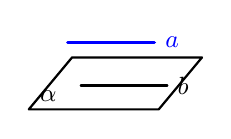
\begin{tikzpicture}[scale=0.55,>=Stealth,line join=round,line cap=round]
  \draw[thick] (0,0)--(3.0,0)--(4.0,1.2)--(1.0,1.2)--cycle;
  \node at (0.45,0.3){\small $\alpha$};
  \draw[thick] (1.2,0.55)--(3.2,0.55) node[right]{\small $b$};
  \draw[very thick,blue] (0.9,1.55)--(2.9,1.55) node[right]{\small $a$};
\end{tikzpicture}}

\begin{paracol}{2}
\teachblock{标准结论}{\textbf{答案 A（(1)(5)）}。(1) 平行公理 4 正确；(5) 线面平行判定定理正确。}
\switchcolumn
\teachblock{错项点拨}{(2) 两线可异面；(3) 中 $a$ 可能在 $\alpha$ 内；(4) 两平面可能相交。}
\end{paracol}


% --- 选择 4 ---
\teachquestionheader{选择 4：面面垂直性质的充要判断}
\mcfigurequestion{已知 $l\subset\alpha$，$\alpha\perp\beta$，$\alpha\cap\beta=m$。则“$l\perp m$”是“$l\perp\beta$”的}{
\mcoptions{充分不必要条件}{必要不充分条件}{充要条件}{既不充分也不必要条件}
}{
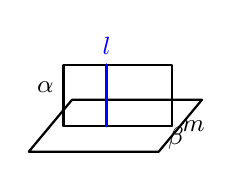
\begin{tikzpicture}[scale=0.55,>=Stealth,line join=round,line cap=round]
  \draw[thick] (0,0)--(3.0,0)--(4.0,1.2)--(1.0,1.2)--cycle;
  \node at (3.4,0.3){\small $\beta$};
  \draw[thick] (0.8,0.6)--(3.3,0.6)--(3.3,2.0)--(0.8,2.0)--cycle;
  \node[left] at (0.8,1.5){\small $\alpha$};
  \draw[thick] (0.8,0.6)--(3.3,0.6) node[right]{\small $m$};
  \draw[very thick,blue] (1.8,0.6)--(1.8,2.0) node[above]{\small $l$};
\end{tikzpicture}}

\begin{paracol}{2}
\teachblock{标准结论}{\textbf{答案 C（充要条件）}。充分性即面面垂直性质定理；必要性由 $l\perp\beta, m\subset\beta \Rightarrow l\perp m$。}
\switchcolumn
\teachblock{重点}{充分性和必要性必须分方向推演，注意已知 $l\subset\alpha$ 这一前提条件。}
\end{paracol}


% --- 选择 5 ---
\teachquestionheader{选择 5：必要不充分条件判断}
\mcfigurequestion{设 $m\subset\alpha$。则“$l\perp m$”是“$l\perp\alpha$”的}{
\mcoptions{充分不必要条件}{必要不充分条件}{充要条件}{既不充分也不必要条件}
}{
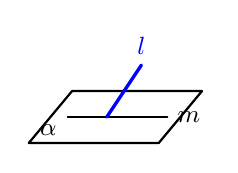
\begin{tikzpicture}[scale=0.55,>=Stealth,line join=round,line cap=round]
  \draw[thick] (0,0)--(3.0,0)--(4.0,1.2)--(1.0,1.2)--cycle;
  \node at (0.45,0.3){\small $\alpha$};
  \draw[thick] (0.9,0.6)--(3.2,0.6) node[right]{\small $m$};
  \draw[very thick,blue] (1.8,0.6)--(2.6,1.8) node[above]{\small $l$};
\end{tikzpicture}}

\begin{paracol}{2}
\teachblock{标准结论}{\textbf{答案 B（必要不充分）}。$l\perp\alpha \Rightarrow l\perp m$（必要）；反之只垂直一条线推不出线面垂直（不充分）。}
\switchcolumn
\teachblock{重点}{强调线面垂直判定必须是“两条相交直线”，一条线不够。}
\end{paracol}


% --- 选择 6 ---
\teachquestionheader{选择 6：平行与垂直混合判断}
\mcfigurequestion{已知 $a,b$ 为两条不同直线，$\alpha,\beta$ 为两个不同平面，下列命题正确的是}{
\mcoptions
{若 $a\parallel b$，$a\parallel\alpha$，则 $b\parallel\alpha$}
{若 $a\parallel b$，$a\perp\alpha$，$b\perp\beta$，则 $\alpha\perp\beta$}
{若 $a\perp\alpha$，$b\perp\beta$，$\alpha\perp\beta$，则 $a\perp b$}
{若 $a\parallel\alpha$，$b\parallel\beta$，$\alpha\perp\beta$，则 $a\perp b$}
}{
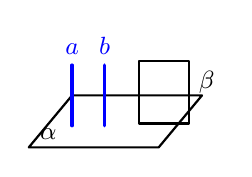
\begin{tikzpicture}[scale=0.55,>=Stealth,line join=round,line cap=round]
  \draw[thick] (0,0)--(3.0,0)--(4.0,1.2)--(1.0,1.2)--cycle;
  \node at (0.45,0.3){\small $\alpha$};
  \draw[thick] (2.55,0.55)--(2.55,2.0)--(3.7,2.0)--(3.7,0.55)--cycle;
  \node[right] at (3.7,1.5){\small $\beta$};
  \draw[very thick,blue] (1.0,0.5)--(1.0,1.9) node[above]{\small $a$};
  \draw[very thick,blue] (1.75,0.5)--(1.75,1.9) node[above]{\small $b$};
\end{tikzpicture}}

\begin{paracol}{2}
\teachblock{标准结论}{\textbf{答案 C}。$a\perp\alpha, b\perp\beta$ 说明直线 $a,b$ 的方向即为两平面的法向量。当 $\alpha\perp\beta$ 时，法向量垂直，故 $a\perp b$。}
\switchcolumn
\teachblock{对比辨析}{B 项错：$a\parallel b$ 推出法向量平行，故 $\alpha\parallel\beta$（而非垂直）；A 项 $b$ 可能在 $\alpha$ 内；D 项方向不确定。}
\end{paracol}


% =====================================================
% 第四板块：平行证明大题（精选代表性大题）
% =====================================================
\section{平行证明代表性大题}

\teachblock{板块方法论}{
平行证明的三条核心路线：
\begin{enumerate}[leftmargin=2em, itemsep=0.1em]
  \item \textbf{直接判定（一条线就够）} $\to$ 在目标平面内找一条与已知直线平行的直线（如中位线）。
  \item \textbf{辅助面面平行（一条线不好找）} $\to$ 补辅助中点，构造平行平面 $\alpha\parallel\beta$，推出线面平行。
\end{enumerate}
}

% --- 大题 1 ---
\teachquestionheader{例 1：四棱锥中证明 $EF\parallel$ 平面 $PAB$（直接判定与辅助中点）}

如图，四棱锥 $P$-$ABCD$ 中，$AB\parallel CD$，$AB\perp AD$，且 $AB=AD=2CD=4$，$PA=2$，$\angle PAB=60^\circ$，直线 $PA$ 与平面 $ABCD$ 所成角为 $30^\circ$，$E,F$ 分别是 $BC$ 和 $PD$ 的中点。

求证：$EF\parallel$ 平面 $PAB$。

\begin{center}
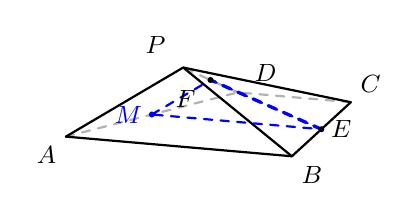
\begin{tikzpicture}[x={(0.92cm,-0.08cm)},y={(0.70cm,0.18cm)},z={(0cm,0.95cm)},>=Stealth,line join=round,line cap=round,scale=0.78]
  \coordinate (A) at (0,0,0);
  \coordinate (B) at (4,0,0);
  \coordinate (D) at (0,4,0);
  \coordinate (C) at (2,4,0);
  \coordinate (P) at (1,{sqrt(2)},1);
  \coordinate (E) at ($(B)!0.5!(C)$);
  \coordinate (F) at ($(P)!0.5!(D)$);
  \coordinate (M) at ($(A)!0.5!(D)$);

  \draw[dashed,thick,gray!60] (A)--(D)--(C);
  \draw[dashed,thick,gray!60] (D)--(P);
  \draw[thick] (A)--(B)--(C);
  \draw[thick] (A)--(P)--(B);
  \draw[thick] (P)--(C);

  \draw[very thick,blue,dashed] (E)--(F);
  \draw[thick,blue,dashed] (M)--(F)--(E)--cycle;

  \node[below left] at (A){\small $A$};
  \node[below right] at (B){\small $B$};
  \node[above right] at (C){\small $C$};
  \node[xshift=10pt,yshift=7pt] at (D){\small $D$};
  \node[xshift=-10pt,yshift=8pt] at (P){\small $P$};
  \fill (E) circle (1.4pt) node[right]{\small $E$};
  \fill (F) circle (1.4pt) node[xshift=-9pt,yshift=-7pt]{\small $F$};
  \fill[blue] (M) circle (1.4pt) node[left]{\small $M$};
\end{tikzpicture}
\end{center}

\begin{paracol}{2}
\teachblock{标准解答}{
取 $AD$ 的中点 $M$，连结 $FM, EM$。

因为 $F, M$ 分别是 $PD, AD$ 的中点，所以 $FM \parallel PA$。

又 $PA\subset$ 平面 $PAB$，$FM\not\subset$ 平面 $PAB$，所以 $FM\parallel$ 平面 $PAB$。

在梯形 $ABCD$ 中，$E, M$ 分别是 $BC, AD$ 的中点，且 $AB\parallel CD$，所以 $EM\parallel AB$。

又 $AB\subset$ 平面 $PAB$，$EM\not\subset$ 平面 $PAB$，所以 $EM\parallel$ 平面 $PAB$。

因为 $FM\cap EM = M$，$FM, EM\subset$ 平面 $EFM$，所以平面 $EFM\parallel$ 平面 $PAB$。

又 $EF\subset$ 平面 $EFM$，所以 $EF\parallel$ 平面 $PAB$。
}

\switchcolumn
\teachblock{教学策略与追问}{
\begin{itemize}
  \item \textbf{突破口}：见到两个中点 $E,F$，顺手在底面边 $AD$ 上再取中点 $M$。
  \item \textbf{关键得分句}：必须明确写出 $FM\parallel PA$ 与 $EM\parallel AB$，并排查 $EFM$ 内两条线相交。
  \item \textbf{得分点提醒}：证明线面平行时，千万不能漏掉“$FM\not\subset$ 平面 $PAB$”。
  \item \textbf{追问}：如果不构造平面 $EFM$，你能直接在平面 $PAB$ 内找一条与 $EF$ 平行的直线吗？（可提示延长 $CD$ 与构造平行四边形）。
\end{itemize}
}
\end{paracol}


\vspace{0.8em}\noindent{\color{rulecolor}\hrule height 0.4pt}\vspace{0.8em}

% --- 大题 2 ---
\teachquestionheader{例 2：矩形底面中证明 $OE\parallel$ 平面 $PCD$（面面平行升阶法）}

在四棱锥 $P$-$ABCD$ 中，四边形 $ABCD$ 是矩形，$\triangle PAD$ 是正三角形，且平面 $PAD\perp$ 平面 $ABCD$，$AB=1$。$O$ 为棱 $AD$ 的中点，$E$ 为棱 $PB$ 的中点。

求证：$OE\parallel$ 平面 $PCD$。

\begin{center}
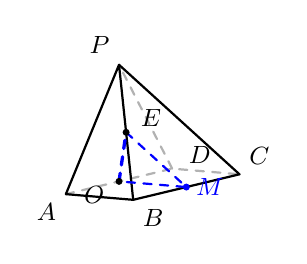
\begin{tikzpicture}[x={(0.95cm,-0.08cm)},y={(0.75cm,0.18cm)},z={(0cm,0.95cm)},>=Stealth,line join=round,line cap=round,scale=0.90]
  \coordinate (A) at (0,0,0);
  \coordinate (B) at (1,0,0);
  \coordinate (D) at (0,2,0);
  \coordinate (C) at (1,2,0);
  \coordinate (P) at (0,1,{sqrt(3)});
  \coordinate (O) at ($(A)!0.5!(D)$);
  \coordinate (E) at ($(P)!0.5!(B)$);
  \coordinate (M) at ($(B)!0.5!(C)$);

  \draw[dashed,thick,gray!60] (A)--(D)--(C);
  \draw[dashed,thick,gray!60] (D)--(P);
  \draw[thick] (A)--(B)--(C);
  \draw[thick] (A)--(P)--(B);
  \draw[thick] (P)--(C);

  \draw[very thick,blue,dashed] (O)--(E);
  \draw[thick,blue,dashed] (E)--(M)--(O);

  \node[below left] at (A){\small $A$};
  \node[below right] at (B){\small $B$};
  \node[above right] at (C){\small $C$};
  \node[xshift=10pt,yshift=5pt] at (D){\small $D$};
  \node[xshift=-7pt,yshift=7pt] at (P){\small $P$};
  \fill (O) circle (1.4pt) node[xshift=-9pt,yshift=-5pt]{\small $O$};
  \fill (E) circle (1.4pt) node[xshift=9pt,yshift=5pt]{\small $E$};
  \fill[blue] (M) circle (1.4pt) node[right]{\small $M$};
\end{tikzpicture}
\end{center}

\begin{paracol}{2}
\teachblock{标准解答}{
取 $PA$ 的中点 $N$，连结 $ON, EN$。（或取 $BC$ 中点 $M$，连结 $OM, EM$）

在 $\triangle PAD$ 中，$O, N$ 分别是 $AD, PA$ 的中点，所以 $ON\parallel PD$。

又 $PD\subset$ 平面 $PCD$，$ON\not\subset$ 平面 $PCD$，所以 $ON\parallel$ 平面 $PCD$。

在 $\triangle PAB$ 中，$E, N$ 分别是 $PB, PA$ 的中点，所以 $EN\parallel AB$。

因为四边形 $ABCD$ 是矩形，所以 $AB\parallel CD$，故 $EN\parallel CD$。

又 $CD\subset$ 平面 $PCD$，$EN\not\subset$ 平面 $PCD$，所以 $EN\parallel$ 平面 $PCD$。

因为 $ON\cap EN = N$，$ON, EN\subset$ 平面 $OEN$，所以平面 $OEN\parallel$ 平面 $PCD$。

又 $OE\subset$ 平面 $OEN$，所以 $OE\parallel$ 平面 $PCD$。
}

\switchcolumn
\teachblock{教学策略与方法升阶}{
\begin{itemize}
  \item \textbf{方法对比}：可以直接取 $PA$ 中点 $N$，也可以取 $BC$ 中点 $M$（构造平行四边形 $OEMC$）。
  \item \textbf{逻辑闭环}：证明 $EN\parallel CD$ 时，必须先写 $EN\parallel AB$，再写矩形给出 $AB\parallel CD$，由平行公理 4 得到 $EN\parallel CD$。
  \item \textbf{易错提醒}：不能跳过 $EN\parallel AB$ 直接写 $EN\parallel CD$。高考批卷对公理 4 的递进要求非常严格。
\end{itemize}
}
\end{paracol}


% =====================================================
% 第五板块：垂直证明代表性大题
% =====================================================
\section{垂直证明代表性大题}

\teachblock{板块方法论}{
垂直证明的三条核心路线：
\begin{enumerate}[leftmargin=2em, itemsep=0.1em]
  \item \textbf{证明线线垂直} $\to$ 转化为证明其中一条线垂直于某个平面（线面垂直性质）。
  \item \textbf{证明线面垂直} $\to$ 找平面内两条相交直线，分别与目标线垂直（线面垂直判定）。
  \item \textbf{证明面面垂直} $\to$ 在其中一个平面内找一条线垂直于另一个平面（面面垂直判定）。
\end{enumerate}
}

% --- 大题 3 ---
\teachquestionheader{例 3：平行四边形与面面垂直性质综合}

在四棱锥 $S$-$ABCD$ 中，平面 $SCD\perp$ 平面 $ABCD$，$SC=SD$。底面 $ABCD$ 是平行四边形，$\angle BAD=\frac{\pi}{3}$，$AB=2$，$AD=1$。$M,N$ 分别为线段 $CD,AB$ 的中点。

求证：$BD\perp$ 平面 $SMN$。

\begin{center}
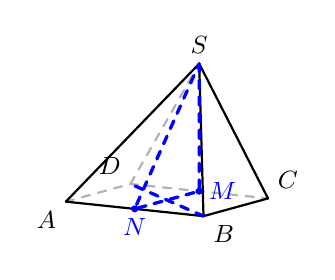
\begin{tikzpicture}[spatial,scale=0.92]
  \coordinate (A) at (0,0,0);
  \coordinate (B) at (2,0,0);
  \coordinate (D) at ({1/2},{sqrt(3)/2},0);
  \coordinate (C) at ({5/2},{sqrt(3)/2},0);
  \coordinate (M) at ({3/2},{sqrt(3)/2},0);
  \coordinate (N) at (1,0,0);
  \coordinate (S) at ({3/2},{sqrt(3)/2},2);

  \draw[dashed,thick,gray!60] (A)--(D)--(C);
  \draw[dashed,thick,gray!60] (D)--(S);
  \draw[thick] (A)--(B)--(C)--(S);
  \draw[thick] (A)--(S)--(B);

  \draw[very thick,blue,dashed] (B)--(D);
  \draw[very thick,blue,dashed] (S)--(M)--(N)--(S);

  \node[below left] at (A){\small $A$};
  \node[below right] at (B){\small $B$};
  \node[above right] at (C){\small $C$};
  \node[above left] at (D){\small $D$};
  \node[above] at (S){\small $S$};
  \fill[blue] (M) circle (1.4pt) node[right]{\small $M$};
  \fill[blue] (N) circle (1.4pt) node[below]{\small $N$};
\end{tikzpicture}
\end{center}

\begin{paracol}{2}
\teachblock{标准解答}{
在 $\triangle SCD$ 中，因为 $SC=SD$，$M$ 为 $CD$ 的中点，所以 $SM\perp CD$。

因为平面 $SCD\perp$ 平面 $ABCD$，平面 $SCD\cap$ 平面 $ABCD = CD$，$SM\subset$ 平面 $SCD$，所以由面面垂直性质定理，得 $SM\perp$ 平面 $ABCD$。

又 $BD\subset$ 平面 $ABCD$，所以 $SM\perp BD$。

在平行四边形 $ABCD$ 中，$M,N$ 分别为 $CD,AB$ 的中点，所以 $MN\parallel AD$ 且 $MN=AD=1$。

在 $\triangle ABD$ 中，$AB=2, AD=1, \angle BAD=60^\circ$，由余弦定理：
\[
  BD^2 = AB^2 + AD^2 - 2AB\cdot AD\cos 60^\circ = 4 + 1 - 2\times 2\times 1\times \frac12 = 3.
\]
因为 $AD^2 + BD^2 = 1 + 3 = 4 = AB^2$，所以由勾股定理逆定理得 $AD\perp BD$。

又 $MN\parallel AD$，所以 $MN\perp BD$。

因为 $SM\cap MN = M$，$SM, MN\subset$ 平面 $SMN$，所以 $BD\perp$ 平面 $SMN$。
}

\switchcolumn
\teachblock{教学策略与关键步}{
\begin{itemize}
  \item \textbf{第一条垂直线（$SM\perp BD$）}：来自“等腰三角形 $SCD$ 中线 $SM\perp CD$” + “面面垂直性质定理”。
  \item \textbf{第二条垂直线（$MN\perp BD$）}：来自“平行四边形中点平行性 $MN\parallel AD$” + “$\triangle ABD$ 勾股逆定理 $AD\perp BD$”。
  \item \textbf{得分句检查}：必须指出 $SM, MN$ 在平面 $SMN$ 内且相交于点 $M$。
\end{itemize}
}
\end{paracol}


\vspace{0.8em}\noindent{\color{rulecolor}\hrule height 0.4pt}\vspace{0.8em}

% --- 大题 4 ---
\teachquestionheader{例 4：数量关系反推与综合线面垂直证明}

四棱锥 $P$-$ABCD$ 的底面 $ABCD$ 是边长为 $2$ 的正方形，平面 $PAB\perp$ 平面 $ABCD$，平面 $PAD\perp$ 平面 $ABCD$。$E$ 为 $PD$ 的中点，三棱锥 $P$-$ACE$ 的体积为 $\frac23$。

求证：$AE\perp$ 平面 $PCD$。

\begin{center}
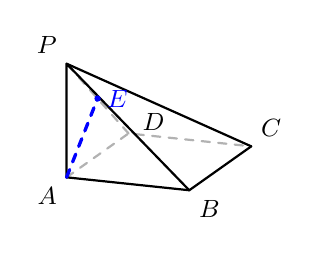
\begin{tikzpicture}[spatial,scale=0.82]
  \coordinate (A) at (0,0,0);
  \coordinate (B) at (2,0,0);
  \coordinate (D) at (0,2,0);
  \coordinate (C) at (2,2,0);
  \coordinate (P) at (0,0,2);
  \coordinate (E) at ($(P)!0.5!(D)$);

  \draw[dashed,thick,gray!60] (A)--(D)--(C);
  \draw[dashed,thick,gray!60] (D)--(P);
  \draw[thick] (A)--(B)--(C);
  \draw[thick] (A)--(P)--(B);
  \draw[thick] (P)--(C);
  \draw[very thick,blue,dashed] (A)--(E);

  \node[below left] at (A){\small $A$};
  \node[below right] at (B){\small $B$};
  \node[above right] at (C){\small $C$};
  \node[xshift=9pt,yshift=4pt] at (D){\small $D$};
  \node[above left] at (P){\small $P$};
  \fill[blue] (E) circle (1.4pt) node[right]{\small $E$};
\end{tikzpicture}
\end{center}

\begin{paracol}{2}
\teachblock{标准解答}{
因为平面 $PAB\perp$ 平面 $ABCD$，平面 $PAD\perp$ 平面 $ABCD$，平面 $PAB\cap$ 平面 $PAD = PA$，由二级结论得 $PA\perp$ 平面 $ABCD$。

设 $PA = h$。在正方形 $ABCD$ 中，$S_{\triangle ACD} = \frac12 \times 2 \times 2 = 2$。

因为 $E$ 为 $PD$ 的中点，所以点 $E$ 到平面 $ABCD$ 的距离为 $\frac h2$。
\[
  V_{P-ACE} = V_{E-PAC} = V_{E-ACD} = \frac13 S_{\triangle ACD} \cdot \frac h2 = \frac13 \times 2 \times \frac h2 = \frac h3.
\]
由 $V_{P-ACE} = \frac23$，得 $\frac h3 = \frac23 \implies h = 2$，即 $PA = 2$。

在 Rt$\triangle PAD$ 中，$PA = AD = 2$，$E$ 为斜边 $PD$ 的中点，所以 $AE\perp PD$。

又因为 $CD\perp AD$，$CD\perp PA$，$AD\cap PA = A$，所以 $CD\perp$ 平面 $PAD$。

因为 $AE\subset$ 平面 $PAD$，所以 $CD\perp AE$，即 $AE\perp CD$。

因为 $PD\cap CD = D$，$PD, CD\subset$ 平面 $PCD$，所以 $AE\perp$ 平面 $PCD$。
}

\switchcolumn
\teachblock{教学策略与方法引申}{
\begin{itemize}
  \item \textbf{第一步：交线垂直}---利用“双侧面垂直底面 $\Rightarrow$ 交线 $PA\perp$ 底面”。
  \item \textbf{第二步：体积反推}---利用 $V_{E-ACD} = \frac13 S \cdot \frac h2$ 算出高 $PA=2$。
  \item \textbf{第三步：两条垂直线}---在 Rt$\triangle PAD$ 中由等腰中线推出 $AE\perp PD$；由 $CD\perp$ 平面 $PAD$ 推出 $CD\perp AE$。
  \item \textbf{得分点检查}：指出 $PD, CD$ 在平面 $PCD$ 内且相交于点 $D$。
\end{itemize}
}
\end{paracol}


% =====================================================
% 第六板块：课堂总结
% =====================================================
\section{课堂总结}

\begin{teachbox}{本讲收束}
最后让学生口述四句话：
\begin{enumerate}[label=\arabic*. , leftmargin=2em, itemsep=0.2em]
  \item 平行证明先找中点和比例点，中位线和面面平行是最常用的两条路线。
  \item 垂直证明先找平面，线面垂直是线线垂直和面面垂直的"桥梁"。
  \item 选择题要特别检查定理前提——"相交""不在面内""在目标平面内"这些词不能省。
  \item 证明题中不要省略关键归属关系，得分句模板要形成肌肉记忆。
\end{enumerate}
\end{teachbox}

\begin{teachbox}{课后复练安排}
\begin{enumerate}[label=\arabic*. , leftmargin=2em, itemsep=0.2em]
  \item 重做例 3，完整写出“等腰中线 + 面面垂直性质 $\to$ 线面垂直判定”的证明链。
  \item 重做例 4，重点落实“体积反推 + 等腰直角三角形 + 线面垂直判定”三步。
  \item 默写线面垂直判定定理的标准得分句（五个前提全部写出）。
\end{enumerate}
\end{teachbox}

\newpage
% =====================================================
% 附录 A：建系与空间直角坐标系（向量法通用体系·课后进阶）
% =====================================================
\appendix
\section{附录 A：建系与空间直角坐标系（向量法通用体系·课后进阶）}

\begin{teachbox}{核心解题理念与最实用的一句话}
\[
  \boxed{\text{\large 先用几何关系造出直角，再用坐标运算解决角度和距离}}
\]
建系不是解题的第一步！第一步永远是观察与识别：哪里有中点、对称轴、等腰三角形、面面垂直，以及第一问已经为第二问提供了什么垂直关系。
\end{teachbox}

\subsection{建系解题的九大核心法则与决策流程}

\teachblock{一、判断是否适合建系}{
出现以下条件时，通常优先选择空间向量建系：
\begin{itemize}[leftmargin=2em, itemsep=0.1em]
  \item 题目中较多垂直关系、长度关系明确；
  \item 目标为求线面角、二面角、点面距离或复杂垂直关系；
  \item 图形中有中点、对称轴、等腰三角形，坐标容易表示。
\end{itemize}
\textbf{反思提醒}：如果只是证明简单的线面垂直，纯几何法往往更简短（3--5 行即可），不必强行建系。
}

\teachblock{二、建系的核心：先找三条两两垂直的方向}{
最常见的建系结构是：
\[
  x\text{ 轴} \perp y\text{ 轴}, \qquad z\text{ 轴} \perp \text{底面}
\]
通常先在底面内找两条互相垂直的直线，再取一条垂直底面的直线作 $z$ 轴。
\begin{enumerate}[label=\arabic*. , leftmargin=2em, itemsep=0.1em]
  \item \textbf{矩形、正方形}：直接利用相邻两边作 $x,y$ 轴；
  \item \textbf{一般菱形}：优先考虑两条对角线作 $x,y$ 轴（除非已知邻边垂直即正方形，否则切忌用邻边）；
  \item \textbf{等腰三角形}：取底边中线垂直底边，作坐标轴；
  \item \textbf{等腰梯形}：优先考虑对称轴和底边作 $x,y$ 轴；
  \item \textbf{面面垂直}：在其中一个平面内作垂直于交线的直线，可推出它垂直于另一个平面（作为 $z$ 轴）。
\end{enumerate}
\textbf{高频失分提醒}：\text{\textbf{图上看着垂直，不代表真的垂直！}}建系前必须在解答中写清楚三轴互相垂直的几何依据。
}

\teachblock{三、原点尽量选在“信息最多”的点}{
坐标原点 $O$ 优先考虑以下“信息中心”：
\[
  \boxed{\text{多条垂线的交点}}
  \quad\succ\quad
  \boxed{\text{底面垂足}}
  \quad\succ\quad
  \boxed{\text{中点/对称中心}}
\]
原点选得好，大量已知点会出现零坐标。例如将底面设在 $z=0$ 平面上，底面所有点的第三坐标均为 $0$。
}

\teachblock{四、坐标轴要顺着图形的特殊几何方向}{
切忌机械地沿着某三条棱建系。更好的选择是：
\begin{itemize}[leftmargin=2em, itemsep=0.1em]
  \item 沿对角线建系（如菱形对角线）；
  \item 沿中线 / 对称轴建系；
  \item 沿第一问证明出的垂线建系。
\end{itemize}
}

\teachblock{五、让未知量尽可能少}{
如果只有一条棱长或一个高度未知，就设为单变量 $a$（如 $P(0,0,a)$），其他点也尽量只用 $a$ 表示。随后用线面角、距离或体积条件建立一个方程求解 $a$。
}

\teachblock{六、图形只差整体尺度且目标为角度时，可归一化}{
当题目给出的条件只确定图形形状、没有固定绝对尺度，且目标只与角度有关时，可以把整个图形按同一比例缩放，设一条基准边长为 1 或 2。
}

\teachblock{七、法向量求解法则与特例}{
已知平面内两个不共线向量 $\boldsymbol{a},\boldsymbol{b}$，设法向量为 $\boldsymbol{n}=(x,y,z)$，列方程组：
\[
  \begin{cases}
    \boldsymbol{n}\cdot\boldsymbol{a} = 0 \\
    \boldsymbol{n}\cdot\boldsymbol{b} = 0
  \end{cases}
\]
令其中一个分量取方便的整数（如 $1$），解出一组简单整数解即可。
}

\teachblock{八、三类空间角公式与高频提醒}{
\begin{enumerate}[label=\arabic*. , leftmargin=2em, itemsep=0.1em]
  \item \textbf{异面直线角}：$\cos\theta = \frac{|\boldsymbol{a}\cdot\boldsymbol{b}|}{\|\boldsymbol{a}\|\|\boldsymbol{b}\|}$；
  \item \textbf{直线与平面角}：$\sin\theta = \frac{|\boldsymbol{v}\cdot\boldsymbol{n}|}{\|\boldsymbol{v}\|\|\boldsymbol{n}\|}$；
  \item \textbf{二面角}：$\cos\varphi = \frac{\boldsymbol{n}_1\cdot\boldsymbol{n}_2}{\|\boldsymbol{n}_1\|\|\boldsymbol{n}_2\|}$。
\end{enumerate}
\textbf{高频提醒}：向量公式 $\cos\varphi = \frac{|\boldsymbol{n}_1\cdot\boldsymbol{n}_2|}{\|\boldsymbol{n}_1\|\|\boldsymbol{n}_2\|}$ 所求为两平面的\textbf{锐角/直角}。若题目要求求具体的二面角，必须结合图形朝向（法向量方向）判断最终取 $\varphi$ 还是 $\pi-\varphi$。
}

\teachblock{九、建完系后先做一次“三项检查”}{
\begin{enumerate}[label=\arabic*. , leftmargin=2em, itemsep=0.1em]
  \item \textbf{三轴垂直检查}：三条坐标轴是否真的两两垂直；
  \item \textbf{坐标比例检查}：各点坐标是否符合边长、比例与中点关系；
  \item \textbf{向量符号检查}：向量终点减起点（$\overrightarrow{AB}=B-A$）方向是否写反。
\end{enumerate}
}

\subsection{同题双系对比示范：同一几何体，两种坐标复杂度}

\begin{teachbox}{案例对比：正四棱锥 $P-ABCD$}
设底面正方形边长为 $2$，底面中心为 $O$，高 $PO=2$。下面两幅图使用\textbf{同一种平行投影规则}；坐标轴方向严格对应真实的 $x,y,z$ 方向，因此可以直接比较建系优劣。
\end{teachbox}

\begin{paracol}{2}
\begin{center}
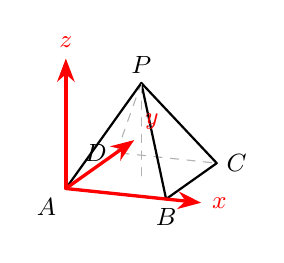
\begin{tikzpicture}[spatial,scale=0.67]
  \coordinate (A) at (0,0,0);
  \coordinate (B) at (2,0,0);
  \coordinate (D) at (0,2,0);
  \coordinate (C) at (2,2,0);
  \coordinate (O) at (1,1,0);
  \coordinate (P) at (1,1,2);
  \draw[dashed,gray!60] (A)--(D)--(C);
  \draw[dashed,gray!60] (D)--(P);
  \draw[thick] (A)--(B)--(C)--(P)--cycle;
  \draw[thick] (B)--(P);
  \draw[dashed,gray!60] (O)--(P);
  \draw[->,red,very thick] (A)--(2.7,0,0) node[right]{\small $x$};
  \draw[->,red,very thick] (A)--(0,2.7,0) node[above right]{\small $y$};
  \draw[->,red,very thick] (A)--(0,0,2.8) node[above]{\small $z$};
  \node[below left] at (A){\small $A$};
  \node[below] at (B){\small $B$};
  \node[right] at (C){\small $C$};
  \node[left] at (D){\small $D$};
  \node[above] at (P){\small $P$};
\end{tikzpicture}
\end{center}
\teachblock{建系 A：以顶点 $A$ 为原点}{
$A(0,0,0)$，$B(2,0,0)$，$C(2,2,0)$，$D(0,2,0)$，$P(1,1,2)$。顶点 $P$ 的三个分量都非零；若后续频繁使用 $P$ 或经过 $P$ 的平面，法向量方程通常更长。
}

\switchcolumn
\begin{center}
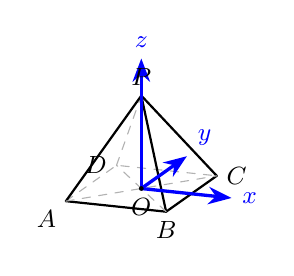
\begin{tikzpicture}[spatial,scale=0.67]
  \coordinate (O) at (0,0,0);
  \coordinate (A) at (-1,-1,0);
  \coordinate (B) at (1,-1,0);
  \coordinate (C) at (1,1,0);
  \coordinate (D) at (-1,1,0);
  \coordinate (P) at (0,0,2);
  \draw[dashed,gray!60] (A)--(D)--(C);
  \draw[dashed,gray!60] (D)--(P);
  \draw[thick] (A)--(B)--(C)--(P)--cycle;
  \draw[thick] (B)--(P);
  \draw[dashed,gray!60] (A)--(C);
  \draw[dashed,gray!60] (B)--(D);
  \draw[dashed,gray!60] (O)--(P);
  \draw[->,blue,very thick] (O)--(1.8,0,0) node[right]{\small $x$};
  \draw[->,blue,very thick] (O)--(0,1.8,0) node[above right]{\small $y$};
  \draw[->,blue,very thick] (O)--(0,0,2.8) node[above]{\small $z$};
  \fill (O) circle (1.3pt) node[below]{\small $O$};
  \node[below left] at (A){\small $A$};
  \node[below] at (B){\small $B$};
  \node[right] at (C){\small $C$};
  \node[left] at (D){\small $D$};
  \node[above] at (P){\small $P$};
\end{tikzpicture}
\end{center}
\teachblock{建系 B（推荐）：以中心 $O$ 为原点}{
$O(0,0,0)$，$A(-1,-1,0)$，$B(1,-1,0)$，$C(1,1,0)$，$D(-1,1,0)$，$P(0,0,2)$。顶点有两个零分量，对称点成对出现 $\pm1$，大量数量积和法向量方程自动消项。
}
\end{paracol}

\end{document}